% =============================================================================
% Project : THE_PHILOSOPHY_OF_VIABILITY
% Book    : Book I — Ontology of Viability
% Book ID : VS.B01
%
% File    : 4_ASSETS/illustrations/
%           VS.B01.P01.C03.S01.SS05.P002.IL01.
%           multiplicity_grouping_and_organization.tex
%
% Asset   : IL01 — Multiplicity, Grouping, and Organization
% Section : 01 — The Ontological Problem of Unity and Plurality
% Chapter : 03 — Unity and Plurality
%
% Purpose :
%   To provide a concrete visual example of different
%   ways in which a plurality of elements may be considered:
%   as distinct elements, as an aggregate, or as an organized
%   composition.
%
% Interpretive Limit :
%   The illustration does not establish the identity,
%   numerical singularity, or ontological unity of any
%   depicted configuration.
%
% Requires (preamble):
%   \usepackage{tikz}
% =============================================================================

\begin{figure}[htbp]
    \centering

    % distance between panel centres (panel width 3.7 cm + gap 0.3 cm)
    \def\pitch{4.0}

    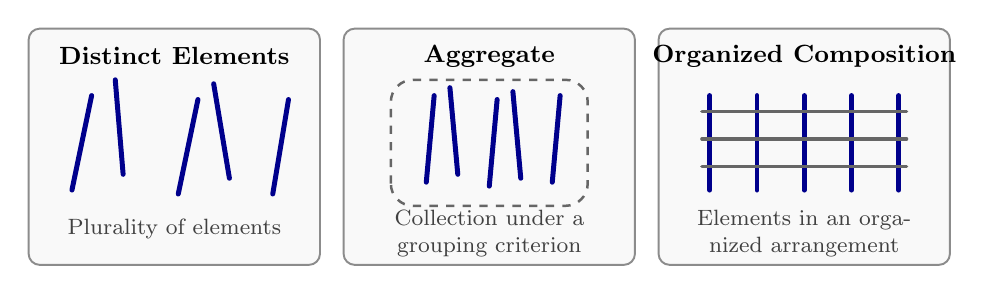
\begin{tikzpicture}[
        font=\small,
        % --- panel frame, title, label ---
        panel/.style={draw=black!45, fill=gray!5, rounded corners=4pt,
                      line width=0.7pt},
        ptitle/.style={font=\small\bfseries, align=center},
        plabel/.style={font=\footnotesize, text=black!75, align=center,
                       text width=3.3cm},
        % --- drawing elements ---
        stick/.style={draw=blue!55!black, line width=1.8pt, line cap=round},
        link/.style={draw=black!60, line width=1.2pt, line cap=round},
        criterion/.style={draw=black!60, dashed, line width=0.9pt,
                          rounded corners=8pt}
    ]

    % ---------------------------------------------------------------
    % Panel 1 — distinct elements (scattered, unconnected, ungrouped)
    % ---------------------------------------------------------------
    \begin{scope}
        \draw[panel] (-1.85,-1.5) rectangle (1.85,1.5);
        \node[ptitle] at (0,1.15) {Distinct Elements};
        \foreach \x/\dx/\y in {-1.30/0.25/-0.55, -0.65/-0.10/-0.35,
                                0.05/0.25/-0.60,  0.70/-0.20/-0.40,
                                1.25/0.20/-0.60} {
            \draw[stick] (\x,\y) -- ++(\dx,1.2);
        }
        \node[plabel] at (0,-1.05) {Plurality of elements};
    \end{scope}

    % ---------------------------------------------------------------
    % Panel 2 — aggregate (same elements, one grouping criterion, no
    % internal connection)
    % ---------------------------------------------------------------
    \begin{scope}[shift={(\pitch,0)}]
        \draw[panel] (-1.85,-1.5) rectangle (1.85,1.5);
        \node[ptitle] at (0,1.15) {Aggregate};
        \foreach \x/\dx/\y in {-0.80/0.10/-0.45, -0.40/-0.10/-0.35,
                                0.00/0.10/-0.50,  0.40/-0.10/-0.40,
                                0.80/0.10/-0.45} {
            \draw[stick] (\x,\y) -- ++(\dx,1.1);
        }
        \draw[criterion] (-1.25,-0.75) rectangle (1.25,0.85);
        \node[plabel] at (0,-1.1) {Collection under a grouping criterion};
    \end{scope}

    % ---------------------------------------------------------------
    % Panel 3 — organized composition (same elements, mutually
    % connected in an arrangement)
    % ---------------------------------------------------------------
    \begin{scope}[shift={(2*\pitch,0)}]
        \draw[panel] (-1.85,-1.5) rectangle (1.85,1.5);
        \node[ptitle] at (0,1.15) {Organized Composition};
        \foreach \x in {-1.2,-0.6,0,0.6,1.2} {
            \draw[stick] (\x,-0.55) -- (\x,0.65);
        }
        \foreach \y in {-0.25,0.10,0.45} {
            \draw[link] (-1.3,\y) -- (1.3,\y);
        }
        \node[plabel] at (0,-1.1) {Elements in an organized arrangement};
    \end{scope}

    \end{tikzpicture}

    \caption{Different Ways of Considering a Plurality of Elements.
    The panels distinguish distinct elements, an aggregate,
    and an organized composition. They illustrate different
    forms of grouping and organization without establishing
    the numerical identity or ontological unity of any
    depicted configuration.}
    \label{fig:multiplicity-grouping-and-organization}
\end{figure}

% =============================================================================
% END OF ASSET IL01 — SECTION 01 OF CHAPTER 03
% =============================================================================